\chapter{Exploration with JASP}

When working with data, one of the first things we do is explore by trying to understand what the data is about, check for patterns, spot unusual values, and get a feel for the numbers before diving into deeper analysis. This step is often called exploratory data analysis (EDA), and it helps us understand what our dataset looks like, what patterns might be hiding in it, and whether anything stands out as unusual or interesting.

Now, you might be thinking:\\
“Can’t we do all this in code using tools like Google Colab or R?”\\
Yes, we absolutely can. But writing code for every single analysis can be time-consuming, especially when we’re just trying to get a quick overview or still learning the basics. Not everyone is comfortable writing code, especially when they are just beginning their journey in data analysis. Sometimes, you just want to take a quick look at the data, run a few simple summaries, and make some graphs  without worrying about syntax or errors. This is where JASP becomes incredibly useful.

\textbf{JASP (Jeffreys’s Amazing Statistics Program)} is a free and open-source software that was built to make statistical analysis easier, faster, and more accessible to everyone. With just a few clicks, you can:

\begin{itemize}
    \item Load datasets and view them in spreadsheet format

    \item Generate descriptive statistics (like mean, median, standard deviation)

    \item Create beautiful visualizations (like histograms, boxplots, and scatterplots)

    \item Run statistical tests (like t-tests, ANOVA, regression, and more)

    \item Explore your data interactively without worrying about code or syntax errors

\end{itemize}

In this chapter, we’ll explore our climate dataset using a tool called JASP. JASP is designed to make data analysis easier and more visual, especially for those who are new to statistics or don’t feel comfortable writing code. You’ll learn how to open your dataset, look at its basic features, and create simple graphs to help you understand what the data is saying.  Even if you’ve never used a statistical tool before, don’t worry, by the end of this chapter, you’ll feel much more confident using JASP to find patterns and insights in your data.

When I first started working with a large climate dataset, I was excited to dive in and start analyzing. But I quickly realized that JASP was having trouble handling such a big file. It would take a while to load, and some actions became really slow. That’s when I decided to take a step back and simplify things a little.

To make the dataset easier to work with, I used Google Colab to filter and simplify it. I selected only the relevant variables and took a smaller sample that still represented the overall data well. This helped reduce the size without losing important information. Once I had a cleaner and more manageable dataset, I moved on to analyzing it in JASP. In this chapter, I’ll walk you through how I cleaned the data using Google Colab and then used JASP to uncover interesting trends and patterns in the climate dataset.

\section*{Filtering the Data in Google Colab}

The following R code was used to filter the climate dataset for analysis in JASP. It includes filtering by date and selecting specific districts.

\begin{verbatim}
# Convert the Date column to proper Date format
df_climate$Date <- as.Date(df_climate$Date, format = "%Y-%m-%d")

# Filter the dataset for the years 2010 to 2019
df_filtered <- df_climate %>%
  filter(lubridate::year(Date) >= 2010 & lubridate::year(Date) <= 2019)

# Further filter for selected districts
df_filtered <- df_filtered %>%
  filter(District %in% c("Kathmandu", "Solukhumbu", "Sarlahi"))

write.csv(df_filtered, "filtered_districts_2010_2019.csv", row.names = FALSE)
\end{verbatim}

\section{Loading the Dataset into JASP}
Once the filtered dataset was ready and saved as a .csv file, I loaded it into JASP to begin the analysis. Here's how you can do the same:

\begin{enumerate}
\item \textbf{Open JASP}\\
Launch the JASP software on your computer. If you haven’t installed it yet, you can download it from \url{https://jasp-stats.org}.

\item \textbf{Open your dataset} \\
From the menu bar, click on \texttt{File > Open > Computer}, then browse and select your saved \texttt{.csv} file (e.g., \texttt{climate\_filtered.csv}).

\item \textbf{View your data} \\
Once the file is opened, the dataset will appear in spreadsheet format. Each column represents a variable (e.g., District, Year, Temp\_2m), and each row is an observation.

\item \textbf{Check variable types}\\
JASP automatically assigns variable types (e.g., nominal, ordinal, scale). You can see these as small icons next to column headers. Make sure they are correct:
\begin{itemize}
    \item \textbf{Scale} (ruler icon): Used for numeric variables where calculations like mean or standard deviation make sense, e.g., \texttt{Temp\_2m} or \texttt{Precipitation}.
    
    \item \textbf{Ordinal} (bars with order): Used for categorical variables that have a meaningful order but not a fixed numerical difference between values, such as \texttt{Month} or \texttt{Education level}.
    
    \item \textbf{Nominal} (venn diagram icon): Used for categorical variables with no natural order, such as \texttt{District}, \texttt{Gender}, or \texttt{Station\_Name}.
\end{itemize}

\end{enumerate}

\section{Editing Data in JASP}

JASP not only allows you to analyze your data but also offers simple tools to make quick edits directly within the software. This can be very helpful if you notice small errors or want to make adjustments without going back to your original dataset.

Here’s how you can edit your data in JASP:

\begin{enumerate}
    \item \textbf{Access the Edit Mode} \\
    After loading your dataset, look for the \texttt{Edit Data} option at the top left corner. Click to enter edit mode.

% figure here--------------------------
\begin{figure}[h]
\centering
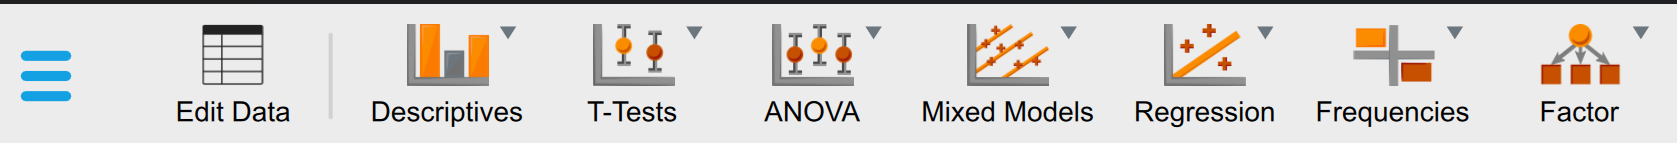
\includegraphics[width=0.7\textwidth]{figures/edit option.png}
\caption{Ribbon Bar}
\end{figure}

\begin{figure}[h]
\centering

\includegraphics[width=0.7\textwidth]{figures/edit mode.png}
\caption{Edit Mode Ribbon Bar}
\end{figure}

    \item \textbf{Modify Data Cells} \\
    In edit mode, you can click on any cell in the dataset and type new values. This is useful for correcting typos, filling in missing data manually, or updating incorrect entries.

    \item \textbf{Rename Variables} \\
    You can also rename columns by clicking on the variable name at the top of each column and typing a new name. This helps make your dataset clearer and easier to understand.

    \item \textbf{Add or Remove Variables} \\
    While editing, you can add new columns for calculated variables or delete unnecessary ones to simplify your dataset.
    The following columns were removed:

\begin{itemize}
    \item \texttt{RH\_2m} (Relative Humidity at 2 meters)
    \item \texttt{WetBulbTemp\_2m} (Wet Bulb Temperature at 2 meters)
    \item \texttt{MaxTemp\_2m} (Maximum Temperature at 2 meters)
    \item \texttt{MinTemp\_2m} (Minimum Temperature at 2 meters)
    \item \texttt{TempRange\_2m} (Temperature Range at 2 meters)
    \item \texttt{EarthSkinTemp} (Temperature of Earth’s Surface)
    \item \texttt{MaxWindSpeed\_10m} (Maximum Wind Speed at 10 meters)
    \item \texttt{MinWindSpeed\_10m} (Minimum Wind Speed at 10 meters)
    \item \texttt{WindSpeedRange\_10m} (Wind Speed Range at 10 meters)
    \item \texttt{MaxWindSpeed\_50m} (Maximum Wind Speed at 50 meters)
    \item \texttt{MinWindSpeed\_50m} (Minimum Wind Speed at 50 meters)
    \item \texttt{WindSpeedRange\_50m} (Wind Speed Range at 50 meters)
\end{itemize}

To make it easier to analyze climate trends over time, I added a new column called \texttt{Year} to the dataset. This column was created by extracting the year from the existing \texttt{Date} column.

\begin{figure}[h]
\centering
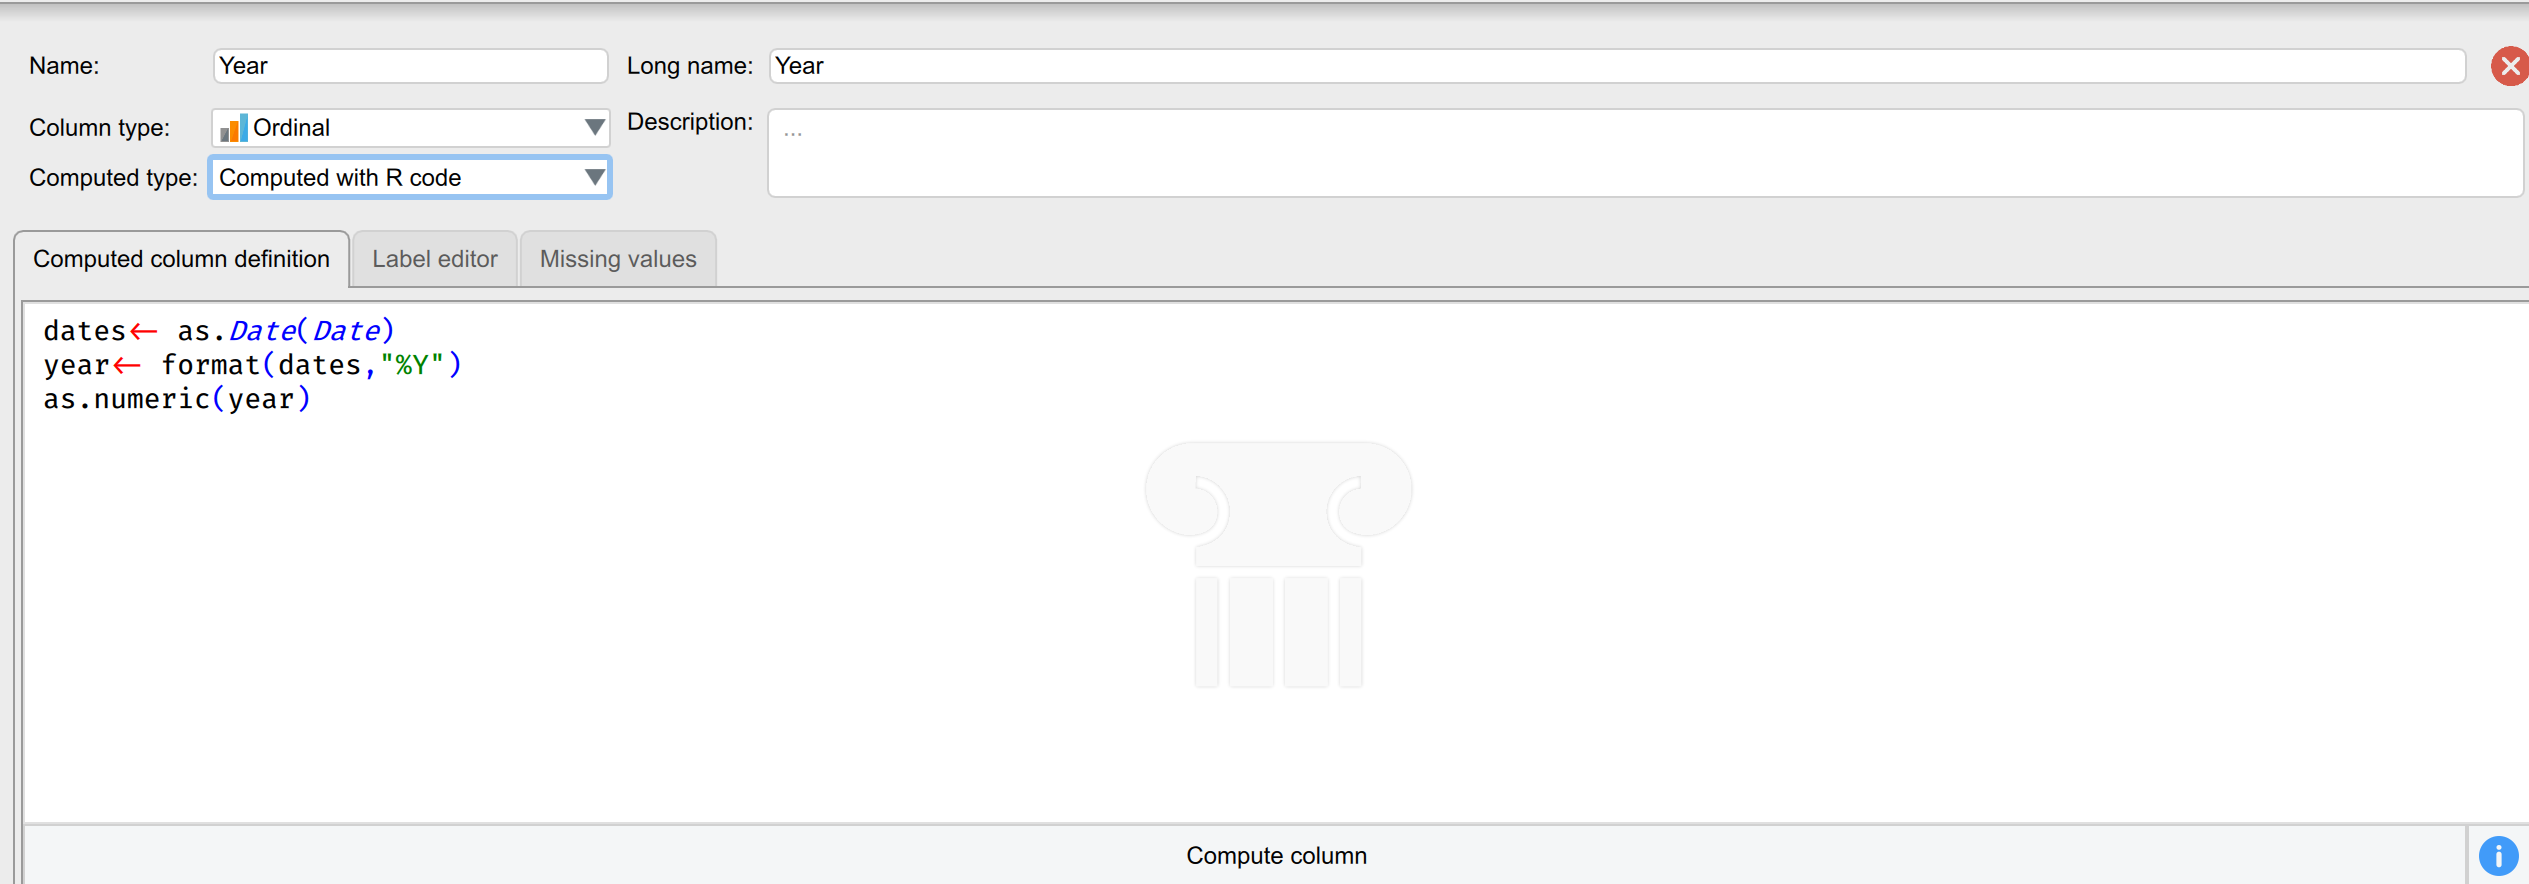
\includegraphics[width=0.7\textwidth]{figures/year_col.png}
\caption{Adding Year Column}
\end{figure}

    \item \textbf{Exit Edit Mode} \\
    When you’re done, click the \texttt{Edit} button again to exit editing and return to analysis mode.

    \item \textbf{Save Your Changes} \\
    Keep in mind, any edits made inside JASP are temporary unless you save your project as a \texttt{.jasp} file. If you reload the original CSV, the edits won’t be preserved.
\end{enumerate}

Editing data directly in JASP can save time and streamline your workflow, especially for quick fixes or small adjustments.

\section{Data Analysis}

With the dataset cleaned, filtered, and properly formatted, it’s time to start exploring the climate data to uncover important patterns and trends. This phase uses JASP’s powerful yet user-friendly tools for descriptive statistics and visualizations, which help us better understand the data before moving to more advanced analyses.
\clearpage

\subsection{Descriptive Statistics}

Descriptive statistics provide a summary of the main features of the data. In JASP, this includes measures such as:

\begin{itemize}
    \item \textbf{Mean} — the average value, e.g., average temperature.
    \item \textbf{Median} — the middle value, which helps understand the distribution.
    \item \textbf{Standard Deviation} — how spread out the data is.
    \item \textbf{Minimum and Maximum} — the range of values observed.
    \item \textbf{Count of Valid and Missing Values} — useful to assess data completeness.
\end{itemize}

Steps:

\begin{enumerate}
    \item Click on descriptives and select descriptive statistics from the drop down menu.
    \item In the left panel, select the variables (e.g., temperature, precipitation, humidity) and move them to the Variables box.
    \item Under the Statistics section, check the options for
    \begin{itemize}
    \item Central Tendency: Mean, Median
    \item Dispersion: Standard Deviation, \item Variance, Range, Interquartile Range (IQR)
Distribution: Skewness, Kurtosis
    \end{itemize}
\end{enumerate}

% figure here--------------------------
\begin{figure}[h]
\centering
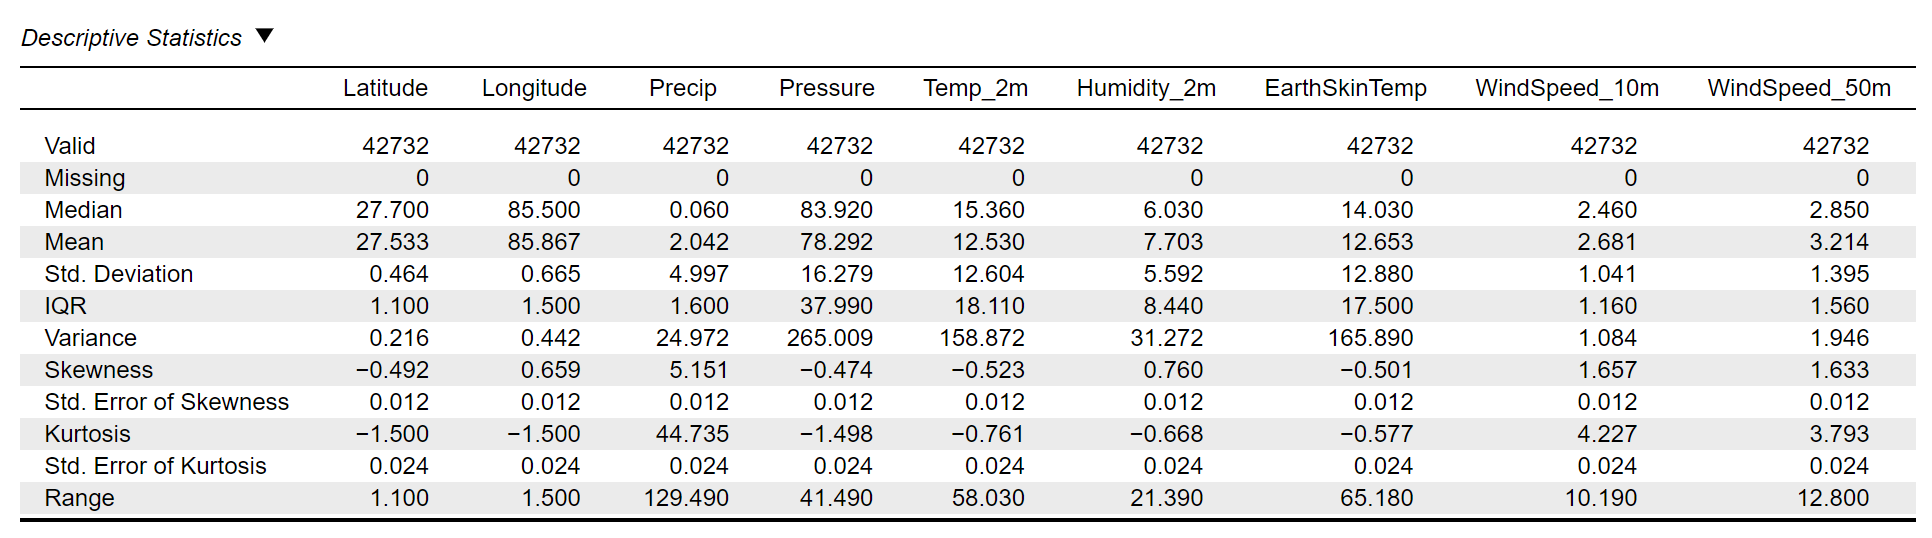
\includegraphics[width=0.7\textwidth]{figures/jasp_descriptivestats.png}
\caption{Descriptive Statistics}
\end{figure}

\textbf{Interpretation:}\\
This table presents key statistics of climate variables:

\begin{itemize}
    \item Sample size is 42,732 with no missing data.
    \item Mean temperature (12.5°C) is lower than median (15.36°C), indicating skew.
    \item Precipitation is low on average (2.04 mm) but with occasional heavy events (max 129.49 mm).
    \item Temperature and precipitation show moderate variability (SD ~12.6 and ~5.0).
    \item Negative skewness in temperature; positive skewness and higher kurtosis in precipitation and wind speed suggest occasional extremes.
\end{itemize}

To visually interpret the Descriptive Statistics, you can use the following graphical representations in JASP:

\subsection*{Histograms for distribution analysis}

Steps to generate histogram in JASP:

\begin{enumerate}
    \item Click Analyses $\rightarrow$ Descriptives $\rightarrow$ Descriptive statistics
    \item Select the variables
    \item Under Frequency Plots, check Histogram.
\end{enumerate}

\begin{figure}[h]
\centering
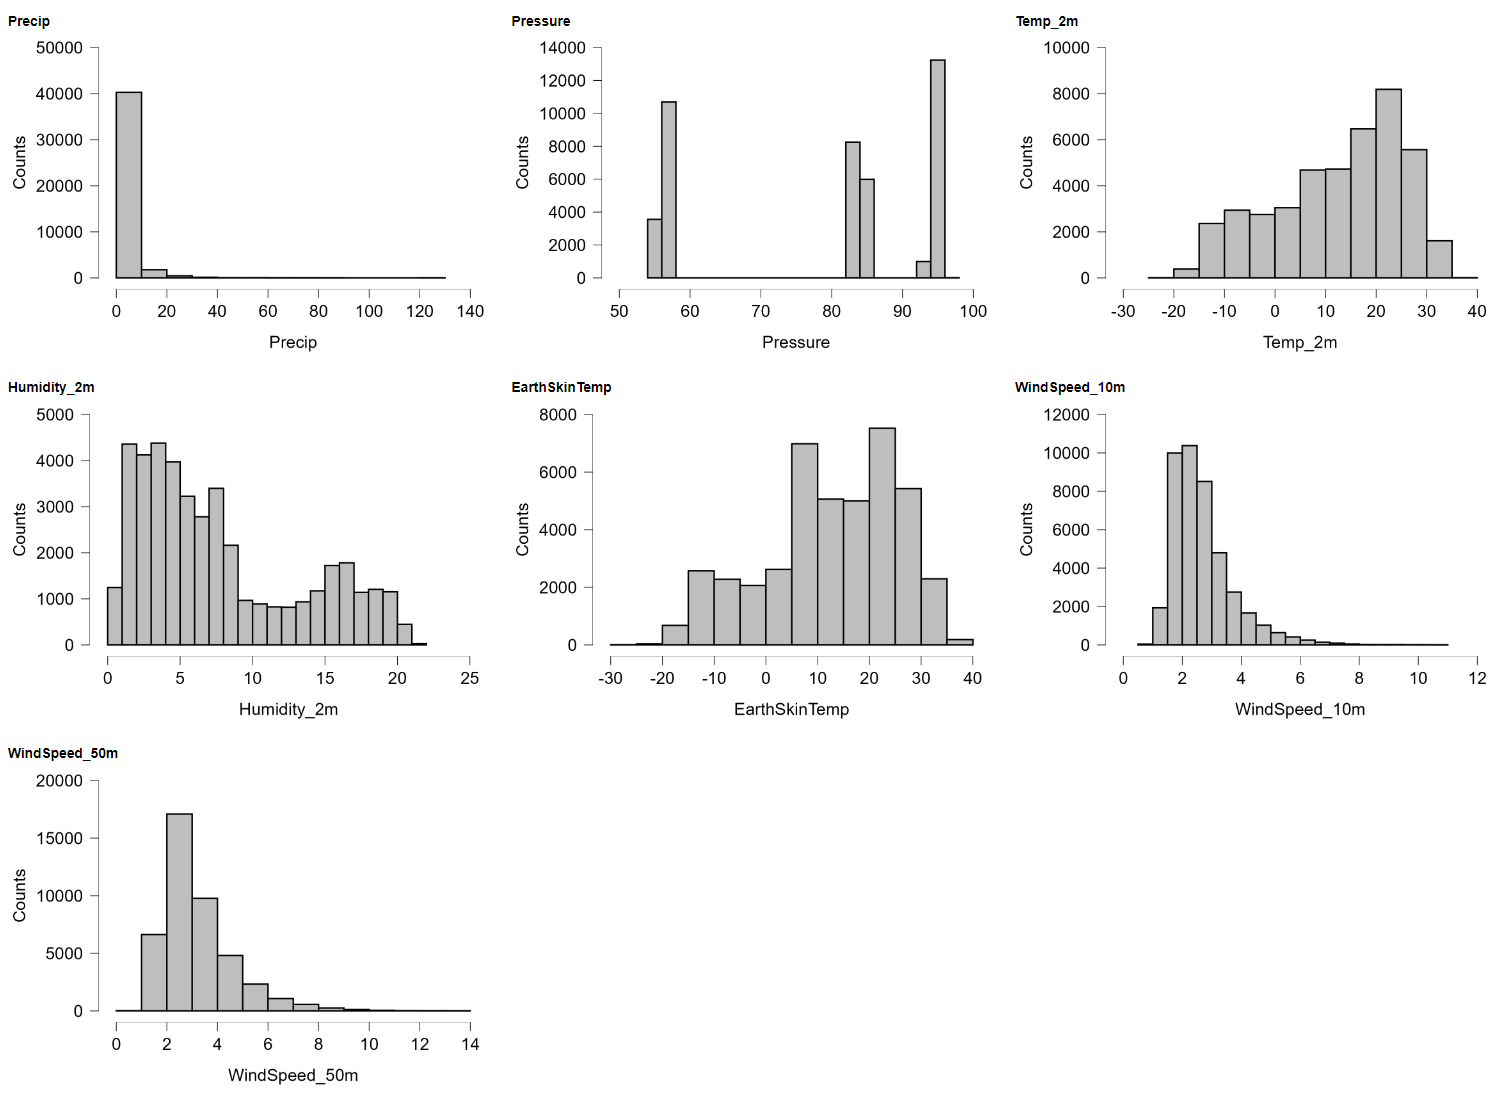
\includegraphics[width=0.7\textwidth]{figures/histogram.png}
\caption{Histogram plot}
\end{figure}

\subsection*{Boxplot}

Boxplots for outlier detection Steps to Generate Boxplots in JASP:
\begin{enumerate}
    \item Click Analyses $\rightarrow$ Descriptives $\rightarrow$ Descriptive statistics
    \item Select the variables
    \item Under Customizable Plots, check Boxplot

\end{enumerate}

\begin{figure}[h]
\centering
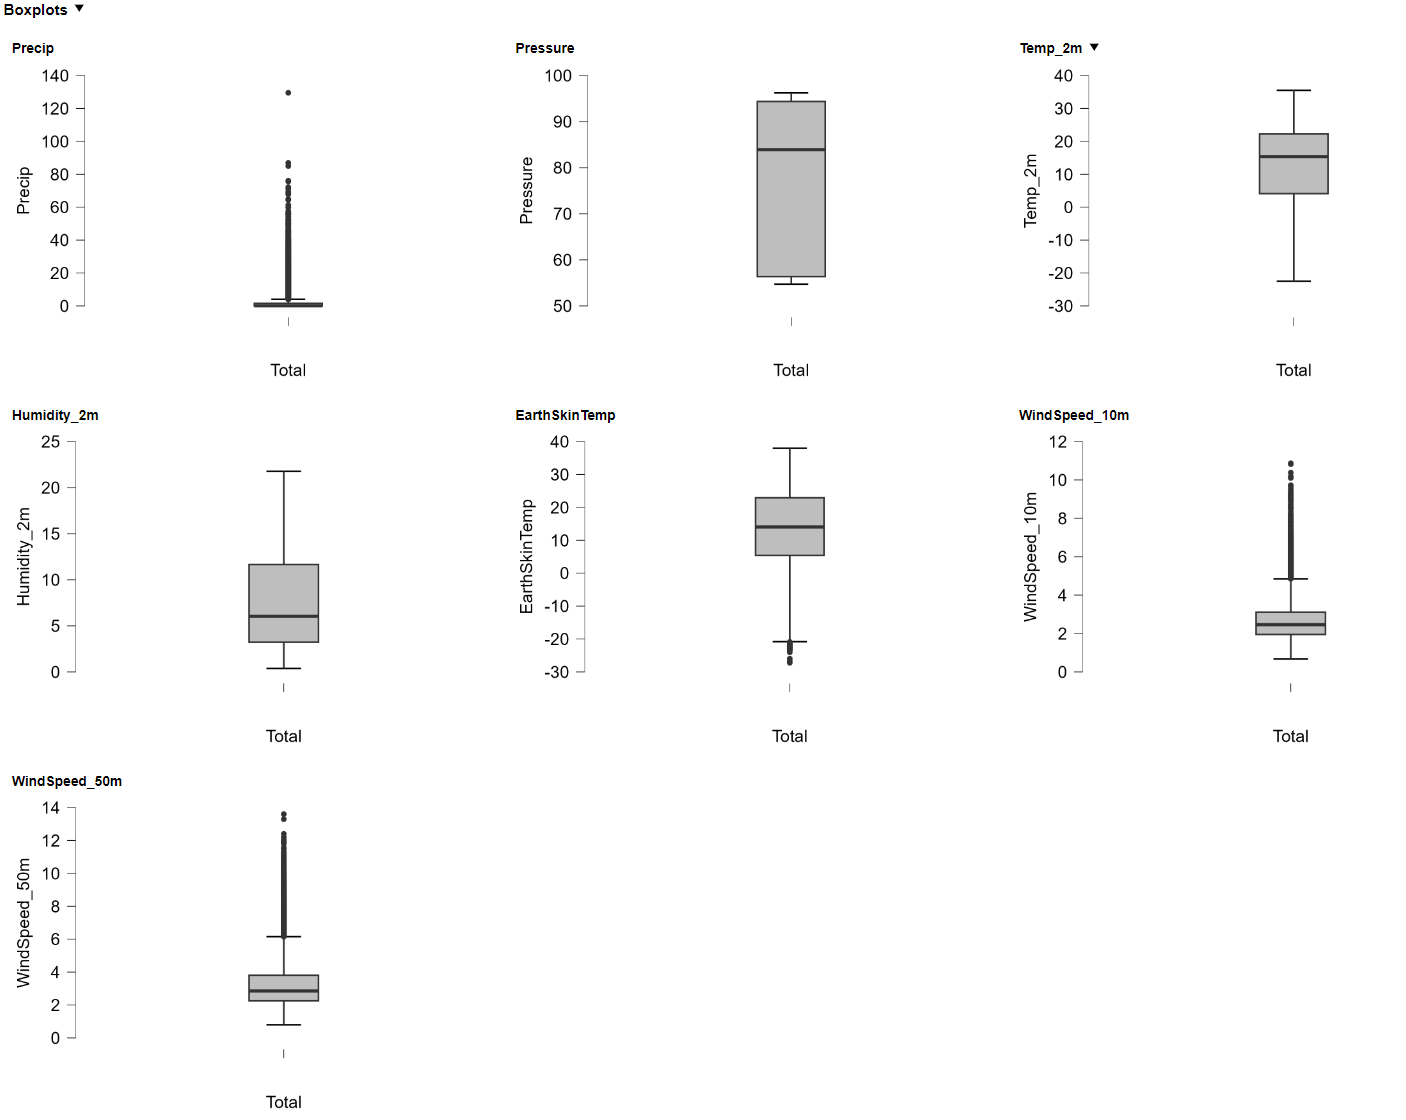
\includegraphics[width=0.7\textwidth]{figures/boxplot.png}
\caption{Boxplot}
\end{figure}

\clearpage
\subsection{Correlation and Heatmap}

\begin{enumerate}
    \item Click on regression and select correlation from the drop down menu under classical.
    \item In the left panel, select the variables and move them to the Variables box.
    \item Check pearson’s correlation and heatmap.
\end{enumerate}

% Figure here-----------------------------
\begin{figure}[h]
\centering
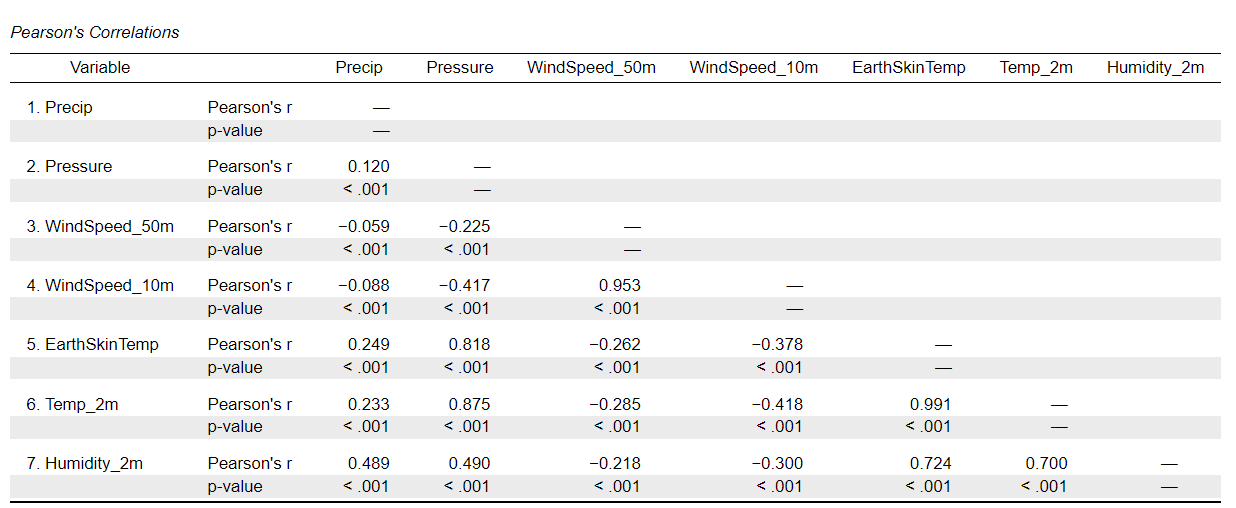
\includegraphics[width=0.7\textwidth]{figures/corr_jasp.png}
\caption{Pearson Correlation Matrix}
\end{figure}

% Figure here-----------------------------
\begin{figure}[h]
\centering
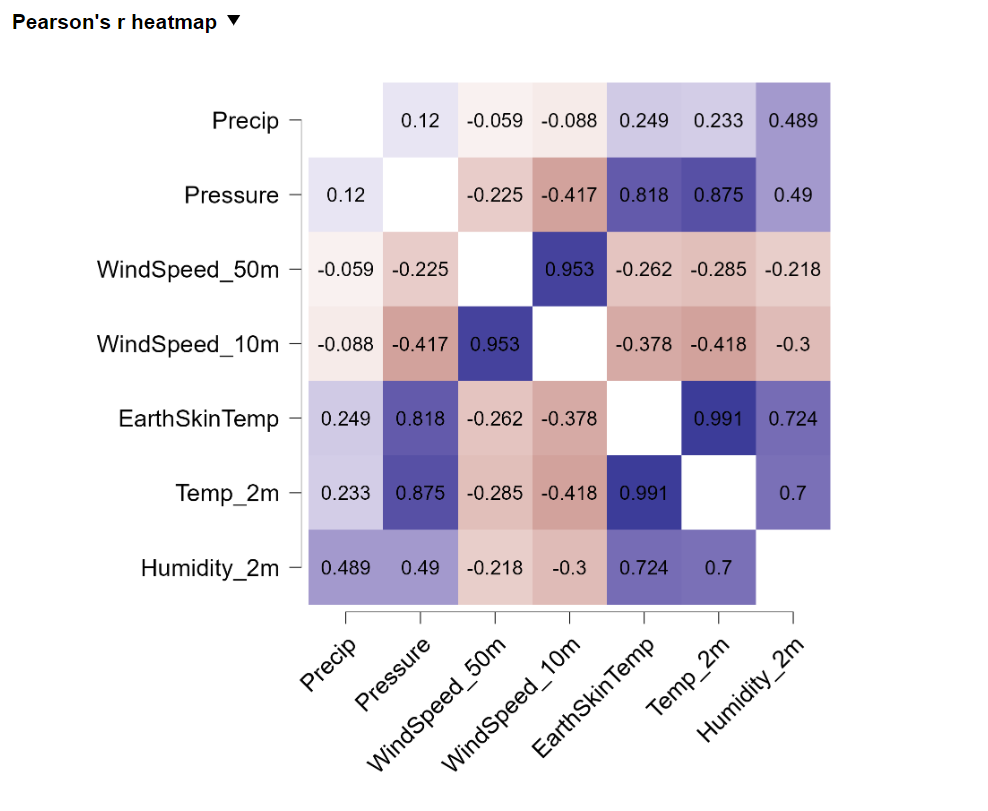
\includegraphics[width=0.7\textwidth]{figures/heatmap_jasp.png}
\caption{Heatmap}
\end{figure}

\clearpage
\subsection{Linear Regression}

Linear Regression is a statistical technique used to model the relationship between a dependent variable (Y) and one or more independent variables (X). It helps us understand how the dependent variable changes when the independent variables change. This method is commonly used in predictive analytics and inferential statistics.

\subsection*{Key Concepts}

\begin{itemize}
    \item \textbf{R\textsuperscript{2} (R-Squared):} R² measures the proportion of variance in the dependent variable that is explained by the independent variables in the model. Think of R² as a score from 0 to 1 that tells you how well your model fits the data.
    \begin{itemize}
        \item An R² of 0.80 means your model explains 80\% of the changes in the result (e.g., temperature). 
        \item The closer to 1, the better your model is at predicting.
    \end{itemize}

    \item \textbf{p-value:} The p-value tests the null hypothesis that a coefficient is equal to zero (i.e., no effect). A value less than 0.05 typically indicates statistical importance. The p-value tells you how likely it is that the result happened by chance.
    \begin{itemize}
        \item If it’s less than 0.05, the variable likely has a real effect on the result. 
        \item For example, a p-value of 0.01 means there’s a very low chance that the result is random.
       \end{itemize}
    \item \textbf{$\boldsymbol{\beta}$ Coefficients:} Beta coefficients represent the estimated change in the dependent variable for a one-unit increase in the independent variable, holding other variables constant. This tells you how much the output will go up or down when the input changes.
    \begin{itemize}
        \item If $\beta = 0.6$ for humidity, then for every 1\% rise in humidity, the temperature increases by 0.6°C (assuming other things stay the same). \item Positive $\beta$ means increase, negative $\beta$ means decrease.
      \end{itemize}
    \item \textbf{Residual Plots:} Residual plots show the difference between observed and predicted values. Random scatter suggests a good model fit. A residual plot is like a ``reality check'' for your model.
    \begin{itemize}
        \item It shows how far off your predictions are.
        \item If the errors (dots) are randomly scattered, it means your model is doing a fair job without obvious bias or patterns.
    \end{itemize}

\end{itemize}

\subsection*{Steps to Perform Linear Regression}

\begin{enumerate}
    \item Click on the \textbf{Regression} tab in the top menu.
    \item Select \textbf{Linear Regression} from the dropdown list.
    \item Drag your dependent variable (Y) (e.g., Temperature) into the \textbf{Dependent Variable} box.
    \item Drag one or more independent variables (X) (e.g., Humidity, Pressure, Precipitation) into the \textbf{Covariates} box.
\end{enumerate}

% Figure here-----------------------------
\begin{figure}[h]
\centering
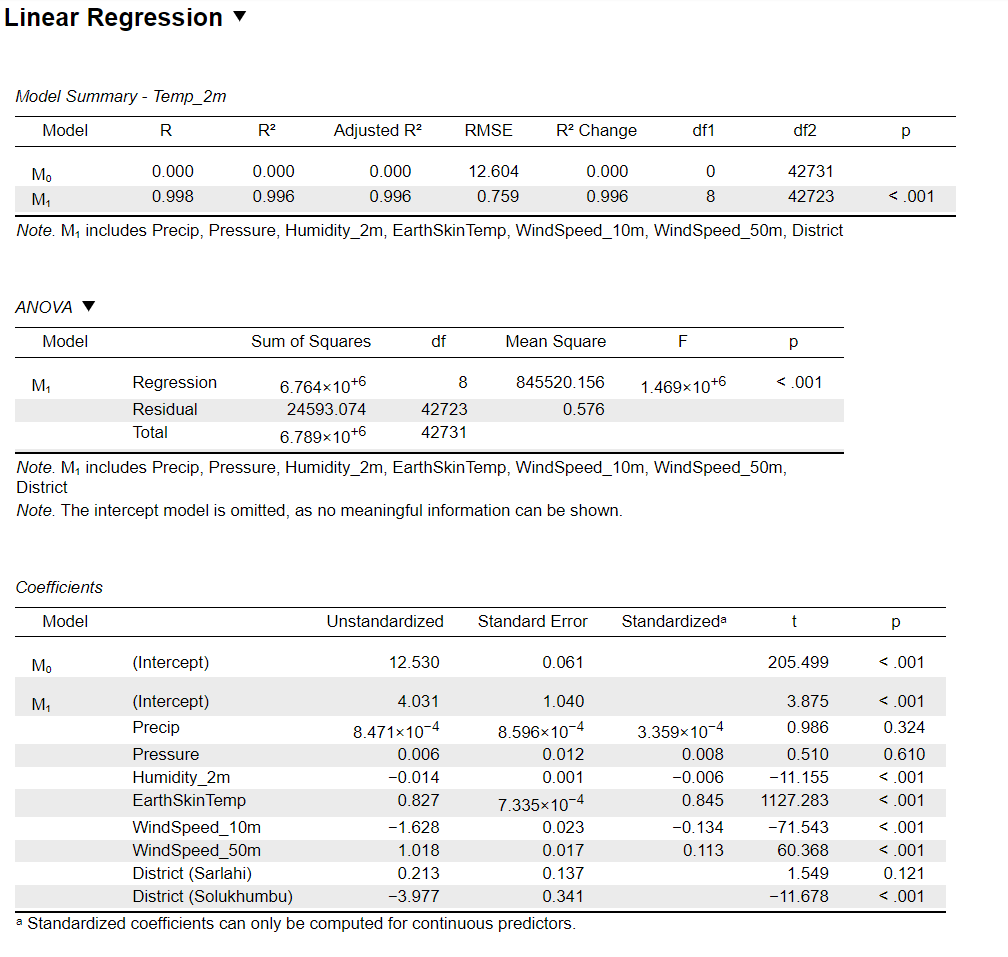
\includegraphics[width=0.7\textwidth]{figures/regression_jasp.png}
\caption{Linear Regression Model Summary}
\end{figure}

\textbf{Interpretation:}
\begin{itemize}
    \item \textbf{Model Summary}
    \begin{itemize}
        \item The model includes 8 predictors: \textit{Precipitation, Pressure, Humidity\_2m, EarthSkinTemp, WindSpeed\_10m, WindSpeed\_50m, District (Sarlahi, Solukhumbu)}.
        \item $R^2 = 0.996$ — the model explains 99.6\% of the variation in temperature.
        \item RMSE (Root Mean Square Error) = 0.759 — the average error in temperature prediction is around $0.76^\circ$C.
        \item The model is statistically significant: $p < .001$.
    \end{itemize}
    \item \textbf{ANOVA Table}
    \begin{itemize}
        \item The model overall is highly significant: $F = 1.469 \times 10^6$, $p < .001$.
        \item This indicates that the combination of predictors meaningfully explains temperature variation.
    \end{itemize}

    \item \textbf{Important Predictors}
    \begin{enumerate}
        \item \textbf{Significant predictors} ($p < .05$):
        \begin{itemize}
            \item EarthSkinTemp — strongest predictor ($t = 1127.283$, $p < .001$)
            \item WindSpeed\_10m and WindSpeed\_50m — both have significant negative effects.
            \item Humidity\_2m — significant negative effect ($p < .001$)
            \item District (Solukhumbu) — significantly colder than the reference district ($t = -11.678$, $p < .001$)
        \end{itemize}
        \item \textbf{Non-significant predictors}:
        \begin{itemize}
            \item Precipitation ($p = 0.324$)
            \item Pressure ($p = 0.610$)
            \item District (Sarlahi) — not significantly different from Kathmandu ($p = 0.121$)
        \end{itemize}
    \end{enumerate}
\end{itemize}

% Figure here-----------------------------
\begin{figure}[h]
\centering
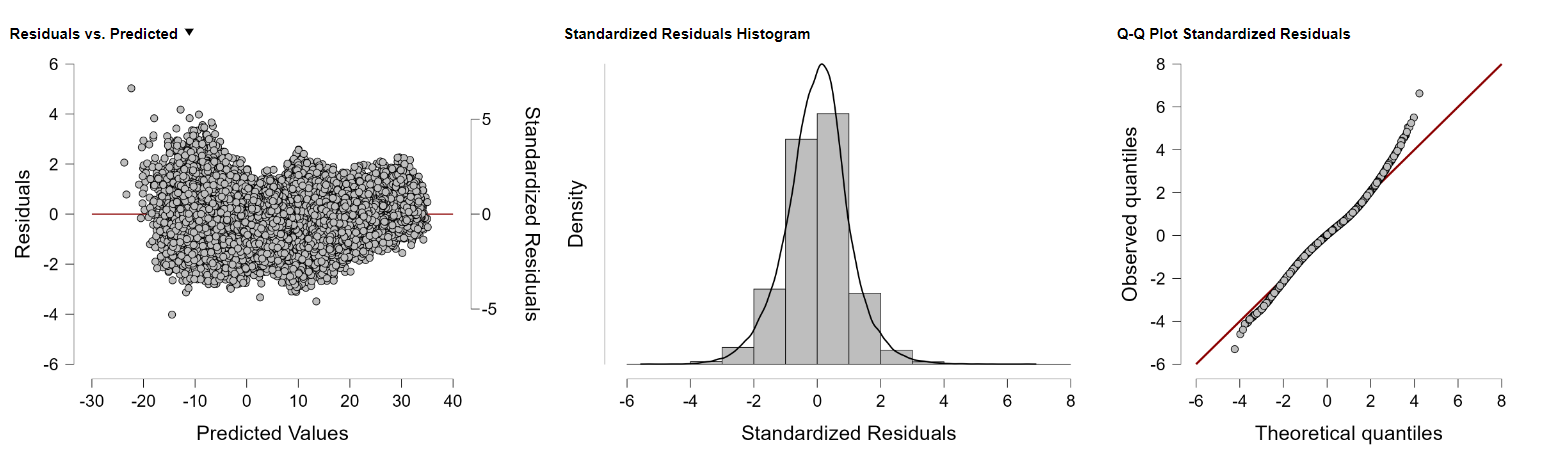
\includegraphics[width=0.7\textwidth]{figures/regression_plot.png}
\caption{Residual Plots}
\end{figure}

\textbf{Residual Diagnostics (Model Assumptions)}
    \begin{itemize}
        \item \textbf{Residuals vs. Predicted}:
        \begin{itemize}
            \item Shows a funnel-shaped spread, suggesting possible heteroscedasticity (non-constant variance).
        \end{itemize}
        \item \textbf{Histogram of Standardized Residuals}:
        \begin{itemize}
            \item Residuals are approximately normally distributed — a good sign.
        \end{itemize}
        \item \textbf{Q-Q Plot}:
        \begin{itemize}
            \item Points follow the straight line closely, indicating residuals are mostly normal, with a few outliers.
        \end{itemize}
    \end{itemize}

The regression model predicts temperature very well using weather and geographic factors. Earth Skin Temperature and Wind Speed are the most important predictors. While the model fits well and errors are mostly normal, the spread of residuals shows a bit of unevenness, which might need attention in further analysis.


\subsection{ANOVA}

ANOVA is a statistical method used to compare the means of multiple groups to see if there are any significant differences among them. It is especially helpful when you have one or more categorical variables (like season or district) and a continuous outcome (like temperature).

\subsection*{Key Concepts}

\begin{itemize}
    \item \textbf{Null Hypothesis (H\textsubscript{0}):} All group means are the same — no real difference between groups.
    
    \item \textbf{Alternative Hypothesis (H\textsubscript{1}):} At least one group mean is different from the others.
    
    \item \textbf{F-Statistic:} This number compares how much the groups differ compared to the variability inside each group. A larger F-value means more likely there is a real difference.
    
    \item \textbf{p-value:} If this value is less than 0.05, we reject the null hypothesis, meaning there is a significant difference between some groups.
    
    \item \textbf{Effect Size ($\eta^2$ or Partial $\eta^2$):} This tells us how much of the change in the dependent variable is explained by the groups — basically, how strong the effect is.

\end{itemize}

\subsection*{How to Perform ANOVA}

\begin{enumerate}
    \item Click on \textbf{ANOVA} from the top menu.
    \item Under \textbf{Classical}, select \textbf{ANOVA}.
    \item Drag your continuous variable (e.g., Temp 2m) into the \textbf{Dependent Variable} box.
    \item Drag your categorical variable(s) (e.g., Season, District) into the \textbf{Fixed Factors} box.
    \item To study interaction effects (how factors work together), select more than one fixed factor (e.g., District × Season).
    \item Choose \textbf{Homogeneity Tests} (like Levene’s test) to check if the groups have similar variances.
    \item Click \textbf{Effect Size ($\eta^2$)} to see the strength of the relationship.
\end{enumerate}

% Figure here-----------------------------
\begin{figure}[h]
\centering
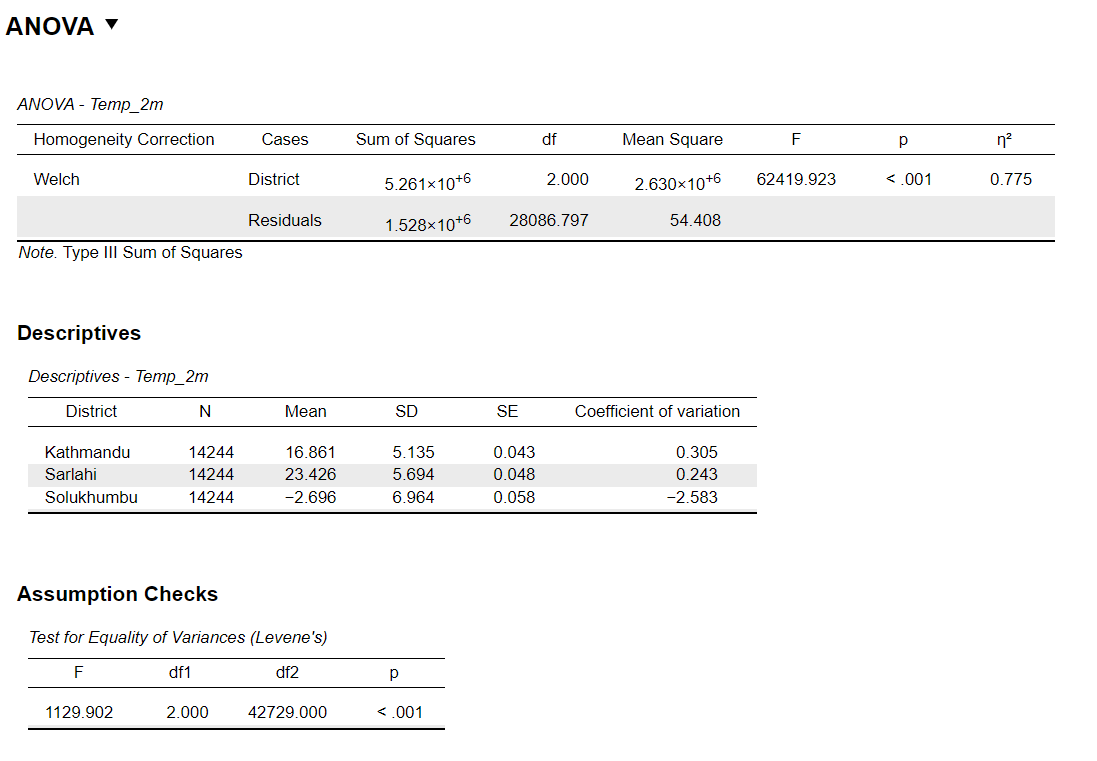
\includegraphics[width=0.7\textwidth]{figures/ANOVA.png}
\caption{ANOVA}
\end{figure}

\textbf{InterPretation:}
\begin{itemize}
    \item \textbf{Main Effect – District}
    \begin{itemize}
        \item Temperature varies significantly across the three districts.
        \item $F = 62{,}419.923$, $p < .001$ — the difference is statistically significant.
        \item $\eta^2 = 0.775$ — very large effect size, meaning 77.5\% of the temperature variation is explained by the district.
    \end{itemize}
    
    \item \textbf{Unexplained (Residual) Variance}
    \begin{itemize}
        \item Some variation in temperature remains unexplained.
        \item Residual sum of squares = $1{,}528{,}000$ (approx).
    \end{itemize}
    
    \item \textbf{Average Temperatures in Each District}
    \begin{itemize}
        \item \textbf{Sarlahi}: Hottest (around $23.4^\circ$C)
        \item \textbf{Kathmandu}: Moderate (around $16.9^\circ$C)
        \item \textbf{Solukhumbu}: Coldest (around $-2.7^\circ$C )(likely due to high elevation)
    \end{itemize}
    
    \item \textbf{Assumption Check(Levene’s Test)}
    \begin{itemize}
        \item $F = 1129.902$, $p < .001$ — indicates variances are not equal across districts.
        \item Because of this, Welch’s ANOVA (which doesn’t require equal variances) was used for better accuracy.
    \end{itemize}
\end{itemize}





